\documentclass[1p]{elsarticle_modified}
%\bibliographystyle{elsarticle-num}

%\usepackage[colorlinks]{hyperref}
%\usepackage{abbrmath_seonhwa} %\Abb, \Ascr, \Acal ,\Abf, \Afrak
\usepackage{amsfonts}
\usepackage{amssymb}
\usepackage{amsmath}
\usepackage{amsthm}
\usepackage{scalefnt}
\usepackage{amsbsy}
\usepackage{kotex}
\usepackage{caption}
\usepackage{subfig}
\usepackage{color}
\usepackage{graphicx}
\usepackage{xcolor} %% white, black, red, green, blue, cyan, magenta, yellow
\usepackage{float}
\usepackage{setspace}
\usepackage{hyperref}

\usepackage{tikz}
\usetikzlibrary{arrows}

\usepackage{multirow}
\usepackage{array} % fixed length table
\usepackage{hhline}

%%%%%%%%%%%%%%%%%%%%%
\makeatletter
\renewcommand*\env@matrix[1][\arraystretch]{%
	\edef\arraystretch{#1}%
	\hskip -\arraycolsep
	\let\@ifnextchar\new@ifnextchar
	\array{*\c@MaxMatrixCols c}}
\makeatother %https://tex.stackexchange.com/questions/14071/how-can-i-increase-the-line-spacing-in-a-matrix
%%%%%%%%%%%%%%%

\usepackage[normalem]{ulem}

\newcommand{\msout}[1]{\ifmmode\text{\sout{\ensuremath{#1}}}\else\sout{#1}\fi}
%SOURCE: \msout is \stkout macro in https://tex.stackexchange.com/questions/20609/strikeout-in-math-mode

\newcommand{\cancel}[1]{
	\ifmmode
	{\color{red}\msout{#1}}
	\else
	{\color{red}\sout{#1}}
	\fi
}

\newcommand{\add}[1]{
	{\color{blue}\uwave{#1}}
}

\newcommand{\replace}[2]{
	\ifmmode
	{\color{red}\msout{#1}}{\color{blue}\uwave{#2}}
	\else
	{\color{red}\sout{#1}}{\color{blue}\uwave{#2}}
	\fi
}

\newcommand{\Sol}{\mathcal{S}} %segment
\newcommand{\D}{D} %diagram
\newcommand{\A}{\mathcal{A}} %arc


%%%%%%%%%%%%%%%%%%%%%%%%%%%%%5 test

\def\sl{\operatorname{\textup{SL}}(2,\Cbb)}
\def\psl{\operatorname{\textup{PSL}}(2,\Cbb)}
\def\quan{\mkern 1mu \triangleright \mkern 1mu}

\theoremstyle{definition}
\newtheorem{thm}{Theorem}[section]
\newtheorem{prop}[thm]{Proposition}
\newtheorem{lem}[thm]{Lemma}
\newtheorem{ques}[thm]{Question}
\newtheorem{cor}[thm]{Corollary}
\newtheorem{defn}[thm]{Definition}
\newtheorem{exam}[thm]{Example}
\newtheorem{rmk}[thm]{Remark}
\newtheorem{alg}[thm]{Algorithm}

\newcommand{\I}{\sqrt{-1}}
\begin{document}

%\begin{frontmatter}
%
%\title{Boundary parabolic representations of knots up to 8 crossings}
%
%%% Group authors per affiliation:
%\author{Yunhi Cho} 
%\address{Department of Mathematics, University of Seoul, Seoul, Korea}
%\ead{yhcho@uos.ac.kr}
%
%
%\author{Seonhwa Kim} %\fnref{s_kim}}
%\address{Center for Geometry and Physics, Institute for Basic Science, Pohang, 37673, Korea}
%\ead{ryeona17@ibs.re.kr}
%
%\author{Hyuk Kim}
%\address{Department of Mathematical Sciences, Seoul National University, Seoul 08826, Korea}
%\ead{hyukkim@snu.ac.kr}
%
%\author{Seokbeom Yoon}
%\address{Department of Mathematical Sciences, Seoul National University, Seoul, 08826,  Korea}
%\ead{sbyoon15@snu.ac.kr}
%
%\begin{abstract}
%We find all boundary parabolic representation of knots up to 8 crossings.
%
%\end{abstract}
%\begin{keyword}
%    \MSC[2010] 57M25 
%\end{keyword}
%
%\end{frontmatter}

%\linenumbers
%\tableofcontents
%
\newcommand\colored[1]{\textcolor{white}{\rule[-0.35ex]{0.8em}{1.4ex}}\kern-0.8em\color{red} #1}%
%\newcommand\colored[1]{\textcolor{white}{ #1}\kern-2.17ex	\textcolor{white}{ #1}\kern-1.81ex	\textcolor{white}{ #1}\kern-2.15ex\color{red}#1	}

{\Large $\underline{12n_{0361}~(K12n_{0361})}$}

\setlength{\tabcolsep}{10pt}
\renewcommand{\arraystretch}{1.6}
\vspace{1cm}\begin{tabular}{m{100pt}>{\centering\arraybackslash}m{274pt}}
\multirow{5}{120pt}{
	\centering
	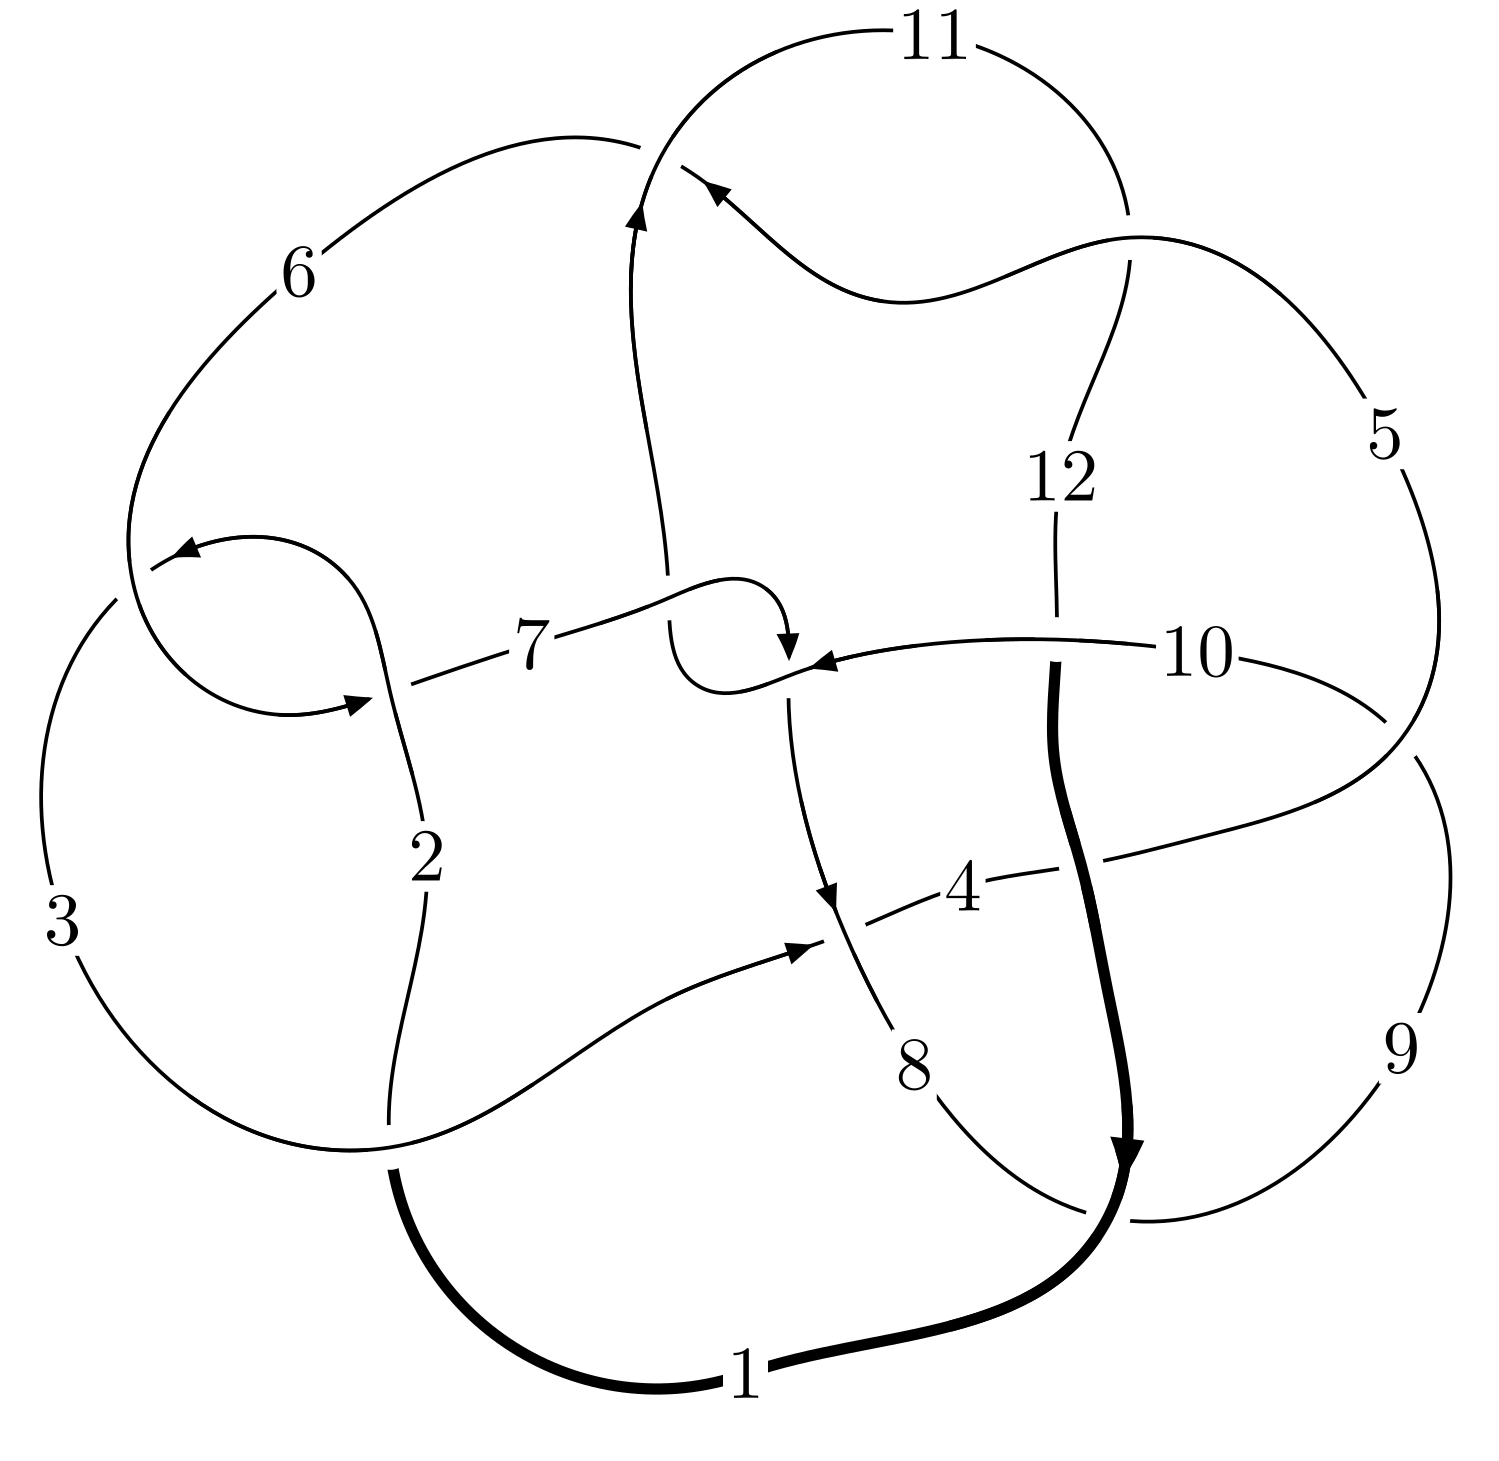
\includegraphics[width=112pt]{../../../GIT/diagram.site/Diagrams/png/2450_12n_0361.png}\\
\ \ \ A knot diagram\footnotemark}&
\allowdisplaybreaks
\textbf{Linearized knot diagam} \\
\cline{2-2}
 &
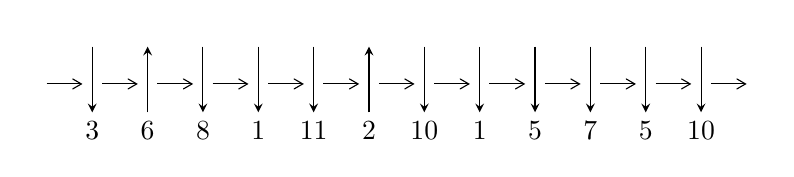
\begin{tikzpicture}[x=20pt, y=17pt]
	% nodes
	\node (C0) at (0, 0) {};
	\node (C1) at (1, 0) {};
	\node (C1U) at (1, +1) {};
	\node (C1D) at (1, -1) {3};

	\node (C2) at (2, 0) {};
	\node (C2U) at (2, +1) {};
	\node (C2D) at (2, -1) {6};

	\node (C3) at (3, 0) {};
	\node (C3U) at (3, +1) {};
	\node (C3D) at (3, -1) {8};

	\node (C4) at (4, 0) {};
	\node (C4U) at (4, +1) {};
	\node (C4D) at (4, -1) {1};

	\node (C5) at (5, 0) {};
	\node (C5U) at (5, +1) {};
	\node (C5D) at (5, -1) {11};

	\node (C6) at (6, 0) {};
	\node (C6U) at (6, +1) {};
	\node (C6D) at (6, -1) {2};

	\node (C7) at (7, 0) {};
	\node (C7U) at (7, +1) {};
	\node (C7D) at (7, -1) {10};

	\node (C8) at (8, 0) {};
	\node (C8U) at (8, +1) {};
	\node (C8D) at (8, -1) {1};

	\node (C9) at (9, 0) {};
	\node (C9U) at (9, +1) {};
	\node (C9D) at (9, -1) {5};

	\node (C10) at (10, 0) {};
	\node (C10U) at (10, +1) {};
	\node (C10D) at (10, -1) {7};

	\node (C11) at (11, 0) {};
	\node (C11U) at (11, +1) {};
	\node (C11D) at (11, -1) {5};

	\node (C12) at (12, 0) {};
	\node (C12U) at (12, +1) {};
	\node (C12D) at (12, -1) {10};
	\node (C13) at (13, 0) {};

	% arrows
	\draw[->,>={angle 60}]
	(C0) edge (C1) (C1) edge (C2) (C2) edge (C3) (C3) edge (C4) (C4) edge (C5) (C5) edge (C6) (C6) edge (C7) (C7) edge (C8) (C8) edge (C9) (C9) edge (C10) (C10) edge (C11) (C11) edge (C12) (C12) edge (C13) ;	\draw[->,>=stealth]
	(C1U) edge (C1D) (C2D) edge (C2U) (C3U) edge (C3D) (C4U) edge (C4D) (C5U) edge (C5D) (C6D) edge (C6U) (C7U) edge (C7D) (C8U) edge (C8D) (C9U) edge (C9D) (C10U) edge (C10D) (C11U) edge (C11D) (C12U) edge (C12D) ;
	\end{tikzpicture} \\
\hhline{~~} \\& 
\textbf{Solving Sequence} \\ \cline{2-2} 
 &
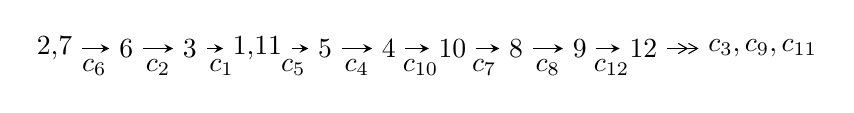
\begin{tikzpicture}[x=23pt, y=7pt]
	% node
	\node (A0) at (-1/8, 0) {2,7};
	\node (A1) at (1, 0) {6};
	\node (A2) at (2, 0) {3};
	\node (A3) at (49/16, 0) {1,11};
	\node (A4) at (33/8, 0) {5};
	\node (A5) at (41/8, 0) {4};
	\node (A6) at (49/8, 0) {10};
	\node (A7) at (57/8, 0) {8};
	\node (A8) at (65/8, 0) {9};
	\node (A9) at (73/8, 0) {12};
	\node (C1) at (1/2, -1) {$c_{6}$};
	\node (C2) at (3/2, -1) {$c_{2}$};
	\node (C3) at (5/2, -1) {$c_{1}$};
	\node (C4) at (29/8, -1) {$c_{5}$};
	\node (C5) at (37/8, -1) {$c_{4}$};
	\node (C6) at (45/8, -1) {$c_{10}$};
	\node (C7) at (53/8, -1) {$c_{7}$};
	\node (C8) at (61/8, -1) {$c_{8}$};
	\node (C9) at (69/8, -1) {$c_{12}$};
	\node (A10) at (11, 0) {$c_{3},c_{9},c_{11}$};

	% edge
	\draw[->,>=stealth]	
	(A0) edge (A1) (A1) edge (A2) (A2) edge (A3) (A3) edge (A4) (A4) edge (A5) (A5) edge (A6) (A6) edge (A7) (A7) edge (A8) (A8) edge (A9) ;
	\draw[->>,>={angle 60}]	
	(A9) edge (A10);
\end{tikzpicture} \\ 

\end{tabular} \\

\footnotetext{
The image of knot diagram is generated by the software ``\textbf{Draw programme}" developed by Andrew Bartholomew(\url{http://www.layer8.co.uk/maths/draw/index.htm\#Running-draw}), where we modified some parts for our purpose(\url{https://github.com/CATsTAILs/LinksPainter}).
}\phantom \\ \newline 
\centering \textbf{Ideals for irreducible components\footnotemark of $X_{\text{par}}$} 
 
\begin{align*}
I^u_{1}&=\langle 
-8.05168\times10^{34} u^{53}+1.07637\times10^{35} u^{52}+\cdots+6.87463\times10^{34} b-6.05852\times10^{33},\\
\phantom{I^u_{1}}&\phantom{= \langle  }1.46995\times10^{35} u^{53}-2.86110\times10^{35} u^{52}+\cdots+6.87463\times10^{34} a+1.14483\times10^{36},\;u^{54}-2 u^{53}+\cdots+7 u+1\rangle \\
I^u_{2}&=\langle 
- u^{17}-2 u^{16}+\cdots+b-2,\;-2 u^{17}- u^{16}+\cdots+a-2 u,\;u^{18}+u^{17}+\cdots+u+1\rangle \\
\\
\end{align*}
\raggedright * 2 irreducible components of $\dim_{\mathbb{C}}=0$, with total 72 representations.\\
\footnotetext{All coefficients of polynomials are rational numbers. But the coefficients are sometimes approximated in decimal forms when there is not enough margin.}
\newpage
\renewcommand{\arraystretch}{1}
\centering \section*{I. $I^u_{1}= \langle -8.05\times10^{34} u^{53}+1.08\times10^{35} u^{52}+\cdots+6.87\times10^{34} b-6.06\times10^{33},\;1.47\times10^{35} u^{53}-2.86\times10^{35} u^{52}+\cdots+6.87\times10^{34} a+1.14\times10^{36},\;u^{54}-2 u^{53}+\cdots+7 u+1 \rangle$}
\flushleft \textbf{(i) Arc colorings}\\
\begin{tabular}{m{7pt} m{180pt} m{7pt} m{180pt} }
\flushright $a_{2}=$&$\begin{pmatrix}0\\u\end{pmatrix}$ \\
\flushright $a_{7}=$&$\begin{pmatrix}1\\0\end{pmatrix}$ \\
\flushright $a_{6}=$&$\begin{pmatrix}1\\u^2\end{pmatrix}$ \\
\flushright $a_{3}=$&$\begin{pmatrix}u\\u^3+u\end{pmatrix}$ \\
\flushright $a_{1}=$&$\begin{pmatrix}u^3\\u^5+u^3+u\end{pmatrix}$ \\
\flushright $a_{11}=$&$\begin{pmatrix}-2.13823 u^{53}+4.16183 u^{52}+\cdots+32.8959 u-16.6530\\1.17122 u^{53}-1.56572 u^{52}+\cdots-4.86988 u+0.0881286\end{pmatrix}$ \\
\flushright $a_{5}=$&$\begin{pmatrix}1.09873 u^{53}-2.43744 u^{52}+\cdots-25.3391 u+18.7511\\-0.466742 u^{53}+0.548863 u^{52}+\cdots+1.52955 u-0.570206\end{pmatrix}$ \\
\flushright $a_{4}=$&$\begin{pmatrix}1.26181 u^{53}-2.68085 u^{52}+\cdots-26.6668 u+18.5566\\-0.318054 u^{53}+0.489820 u^{52}+\cdots+3.00911 u-0.691152\end{pmatrix}$ \\
\flushright $a_{10}=$&$\begin{pmatrix}-0.967010 u^{53}+2.59611 u^{52}+\cdots+28.0260 u-16.5649\\1.17122 u^{53}-1.56572 u^{52}+\cdots-4.86988 u+0.0881286\end{pmatrix}$ \\
\flushright $a_{8}=$&$\begin{pmatrix}-1.33496 u^{53}+2.06007 u^{52}+\cdots+16.5981 u-12.0861\\-0.518639 u^{53}+0.583965 u^{52}+\cdots+0.382552 u+0.726746\end{pmatrix}$ \\
\flushright $a_{9}=$&$\begin{pmatrix}-0.951780 u^{53}+1.73096 u^{52}+\cdots+16.4888 u-12.1502\\-0.301232 u^{53}+0.483930 u^{52}+\cdots+1.35754 u+0.613972\end{pmatrix}$ \\
\flushright $a_{12}=$&$\begin{pmatrix}-3.98736 u^{53}+8.09125 u^{52}+\cdots+69.3422 u-34.0361\\-0.388553 u^{53}+0.437828 u^{52}+\cdots+1.16197 u+1.80831\end{pmatrix}$\\&\end{tabular}
\flushleft \textbf{(ii) Obstruction class $= -1$}\\~\\
\flushleft \textbf{(iii) Cusp Shapes $= -2.52952 u^{53}+4.81017 u^{52}+\cdots+32.1330 u-13.0471$}\\~\\
\newpage\renewcommand{\arraystretch}{1}
\flushleft \textbf{(iv) u-Polynomials at the component}\newline \\
\begin{tabular}{m{50pt}|m{274pt}}
Crossings & \hspace{64pt}u-Polynomials at each crossing \\
\hline $$\begin{aligned}c_{1}\end{aligned}$$&$\begin{aligned}
&u^{54}+20 u^{53}+\cdots-87 u+1
\end{aligned}$\\
\hline $$\begin{aligned}c_{2},c_{6}\end{aligned}$$&$\begin{aligned}
&u^{54}-2 u^{53}+\cdots+7 u+1
\end{aligned}$\\
\hline $$\begin{aligned}c_{3},c_{9}\end{aligned}$$&$\begin{aligned}
&u^{54}- u^{53}+\cdots+10 u-1
\end{aligned}$\\
\hline $$\begin{aligned}c_{4}\end{aligned}$$&$\begin{aligned}
&u^{54}-3 u^{53}+\cdots+16 u+1
\end{aligned}$\\
\hline $$\begin{aligned}c_{5},c_{11}\end{aligned}$$&$\begin{aligned}
&u^{54}+u^{53}+\cdots-200 u-449
\end{aligned}$\\
\hline $$\begin{aligned}c_{7},c_{10}\end{aligned}$$&$\begin{aligned}
&u^{54}-5 u^{53}+\cdots+436 u-41
\end{aligned}$\\
\hline $$\begin{aligned}c_{8}\end{aligned}$$&$\begin{aligned}
&u^{54}+3 u^{53}+\cdots-50452 u-32411
\end{aligned}$\\
\hline $$\begin{aligned}c_{12}\end{aligned}$$&$\begin{aligned}
&u^{54}-5 u^{53}+\cdots-22095 u+889
\end{aligned}$\\
\hline
\end{tabular}\\~\\
\newpage\renewcommand{\arraystretch}{1}
\flushleft \textbf{(v) Riley Polynomials at the component}\newline \\
\begin{tabular}{m{50pt}|m{274pt}}
Crossings & \hspace{64pt}Riley Polynomials at each crossing \\
\hline $$\begin{aligned}c_{1}\end{aligned}$$&$\begin{aligned}
&y^{54}+36 y^{53}+\cdots-6711 y+1
\end{aligned}$\\
\hline $$\begin{aligned}c_{2},c_{6}\end{aligned}$$&$\begin{aligned}
&y^{54}+20 y^{53}+\cdots-87 y+1
\end{aligned}$\\
\hline $$\begin{aligned}c_{3},c_{9}\end{aligned}$$&$\begin{aligned}
&y^{54}-67 y^{53}+\cdots-88 y+1
\end{aligned}$\\
\hline $$\begin{aligned}c_{4}\end{aligned}$$&$\begin{aligned}
&y^{54}-93 y^{53}+\cdots-30 y+1
\end{aligned}$\\
\hline $$\begin{aligned}c_{5},c_{11}\end{aligned}$$&$\begin{aligned}
&y^{54}+25 y^{53}+\cdots+1723672 y+201601
\end{aligned}$\\
\hline $$\begin{aligned}c_{7},c_{10}\end{aligned}$$&$\begin{aligned}
&y^{54}+25 y^{53}+\cdots-41512 y+1681
\end{aligned}$\\
\hline $$\begin{aligned}c_{8}\end{aligned}$$&$\begin{aligned}
&y^{54}-65 y^{53}+\cdots-8887523962 y+1050472921
\end{aligned}$\\
\hline $$\begin{aligned}c_{12}\end{aligned}$$&$\begin{aligned}
&y^{54}-73 y^{53}+\cdots-593861 y+790321
\end{aligned}$\\
\hline
\end{tabular}\\~\\
\newpage\flushleft \textbf{(vi) Complex Volumes and Cusp Shapes}
$$\begin{array}{c|c|c}  
\text{Solutions to }I^u_{1}& \I (\text{vol} + \sqrt{-1}CS) & \text{Cusp shape}\\
 \hline 
\begin{aligned}
u &= -0.782221 + 0.634653 I \\
a &= -0.195755 + 0.247117 I \\
b &= -0.41123 + 1.41581 I\end{aligned}
 & \phantom{-}4.48864 + 3.39067 I & -4.34936 - 2.94495 I \\ \hline\begin{aligned}
u &= -0.782221 - 0.634653 I \\
a &= -0.195755 - 0.247117 I \\
b &= -0.41123 - 1.41581 I\end{aligned}
 & \phantom{-}4.48864 - 3.39067 I & -4.34936 + 2.94495 I \\ \hline\begin{aligned}
u &= -0.977318 + 0.276740 I \\
a &= -0.0878048 - 0.0221906 I \\
b &= \phantom{-}0.424255 + 0.996657 I\end{aligned}
 & -5.26391 - 2.95255 I & -5.80358 + 3.54585 I \\ \hline\begin{aligned}
u &= -0.977318 - 0.276740 I \\
a &= -0.0878048 + 0.0221906 I \\
b &= \phantom{-}0.424255 - 0.996657 I\end{aligned}
 & -5.26391 + 2.95255 I & -5.80358 - 3.54585 I \\ \hline\begin{aligned}
u &= \phantom{-}0.624202 + 0.755472 I \\
a &= \phantom{-}0.453136 + 0.731003 I \\
b &= -0.108485 + 1.364720 I\end{aligned}
 & \phantom{-}3.16221 + 2.63478 I & -6.89633 - 3.54122 I \\ \hline\begin{aligned}
u &= \phantom{-}0.624202 - 0.755472 I \\
a &= \phantom{-}0.453136 - 0.731003 I \\
b &= -0.108485 - 1.364720 I\end{aligned}
 & \phantom{-}3.16221 - 2.63478 I & -6.89633 + 3.54122 I \\ \hline\begin{aligned}
u &= \phantom{-}0.775989 + 0.663204 I \\
a &= -1.14721 - 1.07182 I \\
b &= \phantom{-}1.33969 - 0.51090 I\end{aligned}
 & -5.82772 - 0.87480 I & -6.95939 - 0.10046 I \\ \hline\begin{aligned}
u &= \phantom{-}0.775989 - 0.663204 I \\
a &= -1.14721 + 1.07182 I \\
b &= \phantom{-}1.33969 + 0.51090 I\end{aligned}
 & -5.82772 + 0.87480 I & -6.95939 + 0.10046 I \\ \hline\begin{aligned}
u &= -0.716852 + 0.650173 I \\
a &= \phantom{-}1.11464 - 1.50236 I \\
b &= \phantom{-}0.267394 - 0.730103 I\end{aligned}
 & -6.42976 + 0.18074 I & -5.35993 - 0.34747 I \\ \hline\begin{aligned}
u &= -0.716852 - 0.650173 I \\
a &= \phantom{-}1.11464 + 1.50236 I \\
b &= \phantom{-}0.267394 + 0.730103 I\end{aligned}
 & -6.42976 - 0.18074 I & -5.35993 + 0.34747 I\\
 \hline 
 \end{array}$$\newpage$$\begin{array}{c|c|c}  
\text{Solutions to }I^u_{1}& \I (\text{vol} + \sqrt{-1}CS) & \text{Cusp shape}\\
 \hline 
\begin{aligned}
u &= -0.594108 + 0.867348 I \\
a &= \phantom{-}1.02463 - 1.10108 I \\
b &= -1.340650 + 0.132088 I\end{aligned}
 & -1.16353 - 2.34293 I & -3.59630 + 5.63955 I \\ \hline\begin{aligned}
u &= -0.594108 - 0.867348 I \\
a &= \phantom{-}1.02463 + 1.10108 I \\
b &= -1.340650 - 0.132088 I\end{aligned}
 & -1.16353 + 2.34293 I & -3.59630 - 5.63955 I \\ \hline\begin{aligned}
u &= \phantom{-}0.010981 + 1.054630 I \\
a &= \phantom{-}0.72169 - 1.40947 I \\
b &= -0.409945 + 1.038840 I\end{aligned}
 & -1.20571 + 2.80469 I & -12.64158 - 4.77437 I \\ \hline\begin{aligned}
u &= \phantom{-}0.010981 - 1.054630 I \\
a &= \phantom{-}0.72169 + 1.40947 I \\
b &= -0.409945 - 1.038840 I\end{aligned}
 & -1.20571 - 2.80469 I & -12.64158 + 4.77437 I \\ \hline\begin{aligned}
u &= -0.026887 + 1.056610 I \\
a &= -1.86596 + 0.02219 I \\
b &= \phantom{-}0.945058 - 0.845598 I\end{aligned}
 & -11.48580 - 0.47734 I & -13.44450 + 0. I\phantom{ +0.000000I} \\ \hline\begin{aligned}
u &= -0.026887 - 1.056610 I \\
a &= -1.86596 - 0.02219 I \\
b &= \phantom{-}0.945058 + 0.845598 I\end{aligned}
 & -11.48580 + 0.47734 I & -13.44450 + 0. I\phantom{ +0.000000I} \\ \hline\begin{aligned}
u &= \phantom{-}0.238163 + 1.041600 I \\
a &= -0.453012 + 1.312980 I \\
b &= -0.151747 - 0.544879 I\end{aligned}
 & -0.264943 + 0.782686 I & -8.72185 + 0.87919 I \\ \hline\begin{aligned}
u &= \phantom{-}0.238163 - 1.041600 I \\
a &= -0.453012 - 1.312980 I \\
b &= -0.151747 + 0.544879 I\end{aligned}
 & -0.264943 - 0.782686 I & -8.72185 - 0.87919 I \\ \hline\begin{aligned}
u &= -0.213122 + 0.886225 I \\
a &= \phantom{-}1.87729 - 0.42780 I \\
b &= -0.854175 - 0.507735 I\end{aligned}
 & -2.99097 - 1.86676 I & -15.5248 + 2.2145 I \\ \hline\begin{aligned}
u &= -0.213122 - 0.886225 I \\
a &= \phantom{-}1.87729 + 0.42780 I \\
b &= -0.854175 + 0.507735 I\end{aligned}
 & -2.99097 + 1.86676 I & -15.5248 - 2.2145 I\\
 \hline 
 \end{array}$$\newpage$$\begin{array}{c|c|c}  
\text{Solutions to }I^u_{1}& \I (\text{vol} + \sqrt{-1}CS) & \text{Cusp shape}\\
 \hline 
\begin{aligned}
u &= \phantom{-}0.554630 + 0.711383 I \\
a &= \phantom{-}0.666586 + 0.663185 I \\
b &= -0.632614 - 1.163320 I\end{aligned}
 & \phantom{-}2.75948 - 0.58527 I & -6.51121 - 1.30492 I \\ \hline\begin{aligned}
u &= \phantom{-}0.554630 - 0.711383 I \\
a &= \phantom{-}0.666586 - 0.663185 I \\
b &= -0.632614 + 1.163320 I\end{aligned}
 & \phantom{-}2.75948 + 0.58527 I & -6.51121 + 1.30492 I \\ \hline\begin{aligned}
u &= \phantom{-}0.642108 + 0.935178 I \\
a &= -1.63379 - 0.11874 I \\
b &= \phantom{-}0.101662 - 1.230990 I\end{aligned}
 & \phantom{-}2.59369 + 2.34772 I & -8.00000 + 0. I\phantom{ +0.000000I} \\ \hline\begin{aligned}
u &= \phantom{-}0.642108 - 0.935178 I \\
a &= -1.63379 + 0.11874 I \\
b &= \phantom{-}0.101662 + 1.230990 I\end{aligned}
 & \phantom{-}2.59369 - 2.34772 I & -8.00000 + 0. I\phantom{ +0.000000I} \\ \hline\begin{aligned}
u &= \phantom{-}0.957330 + 0.627734 I \\
a &= -0.0824892 - 0.0033199 I \\
b &= \phantom{-}0.73765 + 1.30778 I\end{aligned}
 & -2.98894 - 8.13870 I & -8.00000 + 3.35962 I \\ \hline\begin{aligned}
u &= \phantom{-}0.957330 - 0.627734 I \\
a &= -0.0824892 + 0.0033199 I \\
b &= \phantom{-}0.73765 - 1.30778 I\end{aligned}
 & -2.98894 + 8.13870 I & -8.00000 - 3.35962 I \\ \hline\begin{aligned}
u &= \phantom{-}0.588547 + 0.982520 I \\
a &= \phantom{-}1.96371 - 0.17505 I \\
b &= -0.758072 + 0.897967 I\end{aligned}
 & \phantom{-}1.85903 + 5.19987 I & -8.00000 - 5.59193 I \\ \hline\begin{aligned}
u &= \phantom{-}0.588547 - 0.982520 I \\
a &= \phantom{-}1.96371 + 0.17505 I \\
b &= -0.758072 - 0.897967 I\end{aligned}
 & \phantom{-}1.85903 - 5.19987 I & -8.00000 + 5.59193 I \\ \hline\begin{aligned}
u &= \phantom{-}0.276388 + 0.802714 I \\
a &= -0.813277 - 0.007279 I \\
b &= \phantom{-}0.173039 + 0.072417 I\end{aligned}
 & -0.465364 + 1.306920 I & -5.27166 - 4.29457 I \\ \hline\begin{aligned}
u &= \phantom{-}0.276388 - 0.802714 I \\
a &= -0.813277 + 0.007279 I \\
b &= \phantom{-}0.173039 - 0.072417 I\end{aligned}
 & -0.465364 - 1.306920 I & -5.27166 + 4.29457 I\\
 \hline 
 \end{array}$$\newpage$$\begin{array}{c|c|c}  
\text{Solutions to }I^u_{1}& \I (\text{vol} + \sqrt{-1}CS) & \text{Cusp shape}\\
 \hline 
\begin{aligned}
u &= -0.838110 + 0.796599 I \\
a &= -0.256450 + 0.157165 I \\
b &= \phantom{-}0.516019 - 1.021330 I\end{aligned}
 & \phantom{-}6.91184 - 0.61269 I & \phantom{-0.000000 } 0 \\ \hline\begin{aligned}
u &= -0.838110 - 0.796599 I \\
a &= -0.256450 - 0.157165 I \\
b &= \phantom{-}0.516019 + 1.021330 I\end{aligned}
 & \phantom{-}6.91184 + 0.61269 I & \phantom{-0.000000 } 0 \\ \hline\begin{aligned}
u &= -0.663079 + 1.010530 I \\
a &= -0.785137 + 1.170500 I \\
b &= \phantom{-}0.347854 + 1.011880 I\end{aligned}
 & -7.52025 - 5.50179 I & \phantom{-0.000000 } 0 \\ \hline\begin{aligned}
u &= -0.663079 - 1.010530 I \\
a &= -0.785137 - 1.170500 I \\
b &= \phantom{-}0.347854 - 1.011880 I\end{aligned}
 & -7.52025 + 5.50179 I & \phantom{-0.000000 } 0 \\ \hline\begin{aligned}
u &= \phantom{-}0.846451 + 0.872894 I \\
a &= -0.251748 - 0.075444 I \\
b &= -0.431221 - 0.973967 I\end{aligned}
 & \phantom{-}3.50126 + 0.93079 I & \phantom{-0.000000 } 0 \\ \hline\begin{aligned}
u &= \phantom{-}0.846451 - 0.872894 I \\
a &= -0.251748 + 0.075444 I \\
b &= -0.431221 + 0.973967 I\end{aligned}
 & \phantom{-}3.50126 - 0.93079 I & \phantom{-0.000000 } 0 \\ \hline\begin{aligned}
u &= \phantom{-}0.691798 + 1.020090 I \\
a &= -0.736000 - 1.034630 I \\
b &= \phantom{-}1.40572 + 0.65983 I\end{aligned}
 & -6.91490 + 6.44905 I & \phantom{-0.000000 } 0 \\ \hline\begin{aligned}
u &= \phantom{-}0.691798 - 1.020090 I \\
a &= -0.736000 + 1.034630 I \\
b &= \phantom{-}1.40572 - 0.65983 I\end{aligned}
 & -6.91490 - 6.44905 I & \phantom{-0.000000 } 0 \\ \hline\begin{aligned}
u &= -0.685621 + 1.030320 I \\
a &= \phantom{-}1.85848 - 0.20635 I \\
b &= -0.56316 - 1.42285 I\end{aligned}
 & \phantom{-}3.29320 - 8.95161 I & \phantom{-0.000000 } 0 \\ \hline\begin{aligned}
u &= -0.685621 - 1.030320 I \\
a &= \phantom{-}1.85848 + 0.20635 I \\
b &= -0.56316 + 1.42285 I\end{aligned}
 & \phantom{-}3.29320 + 8.95161 I & \phantom{-0.000000 } 0\\
 \hline 
 \end{array}$$\newpage$$\begin{array}{c|c|c}  
\text{Solutions to }I^u_{1}& \I (\text{vol} + \sqrt{-1}CS) & \text{Cusp shape}\\
 \hline 
\begin{aligned}
u &= \phantom{-}0.814791 + 0.938243 I \\
a &= \phantom{-}1.082890 + 0.699947 I \\
b &= -0.565715 + 0.957837 I\end{aligned}
 & \phantom{-}3.28563 + 5.26424 I & \phantom{-0.000000 } 0 \\ \hline\begin{aligned}
u &= \phantom{-}0.814791 - 0.938243 I \\
a &= \phantom{-}1.082890 - 0.699947 I \\
b &= -0.565715 - 0.957837 I\end{aligned}
 & \phantom{-}3.28563 - 5.26424 I & \phantom{-0.000000 } 0 \\ \hline\begin{aligned}
u &= -0.783368 + 0.973705 I \\
a &= -1.53300 + 0.36496 I \\
b &= \phantom{-}0.642887 + 0.900173 I\end{aligned}
 & \phantom{-}6.36672 - 5.44538 I & \phantom{-0.000000 } 0 \\ \hline\begin{aligned}
u &= -0.783368 - 0.973705 I \\
a &= -1.53300 - 0.36496 I \\
b &= \phantom{-}0.642887 - 0.900173 I\end{aligned}
 & \phantom{-}6.36672 + 5.44538 I & \phantom{-0.000000 } 0 \\ \hline\begin{aligned}
u &= -0.169579 + 1.266130 I \\
a &= -1.24464 - 0.96277 I \\
b &= \phantom{-}0.714749 + 0.999139 I\end{aligned}
 & -10.81370 - 6.61602 I & \phantom{-0.000000 } 0 \\ \hline\begin{aligned}
u &= -0.169579 - 1.266130 I \\
a &= -1.24464 + 0.96277 I \\
b &= \phantom{-}0.714749 - 0.999139 I\end{aligned}
 & -10.81370 + 6.61602 I & \phantom{-0.000000 } 0 \\ \hline\begin{aligned}
u &= \phantom{-}0.753233 + 1.099800 I \\
a &= -1.82443 - 0.33859 I \\
b &= \phantom{-}0.84183 - 1.33565 I\end{aligned}
 & -4.4657 + 14.4090 I & \phantom{-0.000000 } 0 \\ \hline\begin{aligned}
u &= \phantom{-}0.753233 - 1.099800 I \\
a &= -1.82443 + 0.33859 I \\
b &= \phantom{-}0.84183 + 1.33565 I\end{aligned}
 & -4.4657 - 14.4090 I & \phantom{-0.000000 } 0 \\ \hline\begin{aligned}
u &= -0.564814 + 1.229530 I \\
a &= \phantom{-}0.345121 + 0.886401 I \\
b &= \phantom{-}0.335671 - 0.800648 I\end{aligned}
 & -8.30076 - 2.64729 I & \phantom{-0.000000 } 0 \\ \hline\begin{aligned}
u &= -0.564814 - 1.229530 I \\
a &= \phantom{-}0.345121 - 0.886401 I \\
b &= \phantom{-}0.335671 + 0.800648 I\end{aligned}
 & -8.30076 + 2.64729 I & \phantom{-0.000000 } 0\\
 \hline 
 \end{array}$$\newpage$$\begin{array}{c|c|c}  
\text{Solutions to }I^u_{1}& \I (\text{vol} + \sqrt{-1}CS) & \text{Cusp shape}\\
 \hline 
\begin{aligned}
u &= \phantom{-}0.444579 + 0.121551 I \\
a &= -0.860489 + 0.135214 I \\
b &= -0.187796 + 1.115610 I\end{aligned}
 & \phantom{-}2.66689 + 1.69511 I & -1.25940 - 4.46780 I \\ \hline\begin{aligned}
u &= \phantom{-}0.444579 - 0.121551 I \\
a &= -0.860489 - 0.135214 I \\
b &= -0.187796 - 1.115610 I\end{aligned}
 & \phantom{-}2.66689 - 1.69511 I & -1.25940 + 4.46780 I \\ \hline\begin{aligned}
u &= -0.297162\phantom{ +0.000000I} \\
a &= -0.983290\phantom{ +0.000000I} \\
b &= -0.513330\phantom{ +0.000000I}\end{aligned}
 & -0.837204\phantom{ +0.000000I} & -11.6370\phantom{ +0.000000I} \\ \hline\begin{aligned}
u &= -0.111060\phantom{ +0.000000I} \\
a &= -19.6906\phantom{ +0.000000I} \\
b &= \phantom{-}0.755994\phantom{ +0.000000I}\end{aligned}
 & -7.69304\phantom{ +0.000000I} & -16.8530\phantom{ +0.000000I}\\
 \hline 
 \end{array}$$\newpage\newpage\renewcommand{\arraystretch}{1}
\centering \section*{II. $I^u_{2}= \langle - u^{17}-2 u^{16}+\cdots+b-2,\;-2 u^{17}- u^{16}+\cdots+a-2 u,\;u^{18}+u^{17}+\cdots+u+1 \rangle$}
\flushleft \textbf{(i) Arc colorings}\\
\begin{tabular}{m{7pt} m{180pt} m{7pt} m{180pt} }
\flushright $a_{2}=$&$\begin{pmatrix}0\\u\end{pmatrix}$ \\
\flushright $a_{7}=$&$\begin{pmatrix}1\\0\end{pmatrix}$ \\
\flushright $a_{6}=$&$\begin{pmatrix}1\\u^2\end{pmatrix}$ \\
\flushright $a_{3}=$&$\begin{pmatrix}u\\u^3+u\end{pmatrix}$ \\
\flushright $a_{1}=$&$\begin{pmatrix}u^3\\u^5+u^3+u\end{pmatrix}$ \\
\flushright $a_{11}=$&$\begin{pmatrix}2 u^{17}+u^{16}+\cdots+7 u^2+2 u\\u^{17}+2 u^{16}+\cdots+4 u+2\end{pmatrix}$ \\
\flushright $a_{5}=$&$\begin{pmatrix}u^{16}+u^{15}+\cdots+6 u+1\\- u^{17}- u^{16}+\cdots- u+2\end{pmatrix}$ \\
\flushright $a_{4}=$&$\begin{pmatrix}u^{15}+3 u^{13}+8 u^{11}+13 u^9+17 u^7- u^6+16 u^5+11 u^3-2 u^2+6 u\\- u^{17}- u^{16}+\cdots+u^2+2\end{pmatrix}$ \\
\flushright $a_{10}=$&$\begin{pmatrix}3 u^{17}+3 u^{16}+\cdots+6 u+2\\u^{17}+2 u^{16}+\cdots+4 u+2\end{pmatrix}$ \\
\flushright $a_{8}=$&$\begin{pmatrix}- u^{16}- u^{15}+\cdots-3 u-4\\2 u^{17}+2 u^{16}+\cdots+4 u-1\end{pmatrix}$ \\
\flushright $a_{9}=$&$\begin{pmatrix}- u^{16}- u^{15}+\cdots-3 u-4\\2 u^{17}+2 u^{16}+\cdots+6 u^2+4 u\end{pmatrix}$ \\
\flushright $a_{12}=$&$\begin{pmatrix}u^{17}+u^{16}+\cdots- u+5\\- u^{17}- u^{16}+\cdots-4 u-1\end{pmatrix}$\\&\end{tabular}
\flushleft \textbf{(ii) Obstruction class $= 1$}\\~\\
\flushleft \textbf{(iii) Cusp Shapes $= u^{17}+2 u^{16}+4 u^{15}+7 u^{14}+11 u^{13}+19 u^{12}+22 u^{11}+31 u^{10}+32 u^9+40 u^8+38 u^7+34 u^6+33 u^5+19 u^4+21 u^3+2 u^2+8 u-12$}\\~\\
\newpage\renewcommand{\arraystretch}{1}
\flushleft \textbf{(iv) u-Polynomials at the component}\newline \\
\begin{tabular}{m{50pt}|m{274pt}}
Crossings & \hspace{64pt}u-Polynomials at each crossing \\
\hline $$\begin{aligned}c_{1}\end{aligned}$$&$\begin{aligned}
&u^{18}-7 u^{17}+\cdots-11 u+1
\end{aligned}$\\
\hline $$\begin{aligned}c_{2}\end{aligned}$$&$\begin{aligned}
&u^{18}- u^{17}+\cdots- u+1
\end{aligned}$\\
\hline $$\begin{aligned}c_{3}\end{aligned}$$&$\begin{aligned}
&u^{18}-10 u^{16}+\cdots-4 u+1
\end{aligned}$\\
\hline $$\begin{aligned}c_{4}\end{aligned}$$&$\begin{aligned}
&u^{18}+4 u^{17}+\cdots+10 u+1
\end{aligned}$\\
\hline $$\begin{aligned}c_{5}\end{aligned}$$&$\begin{aligned}
&u^{18}+6 u^{16}+\cdots+4 u+1
\end{aligned}$\\
\hline $$\begin{aligned}c_{6}\end{aligned}$$&$\begin{aligned}
&u^{18}+u^{17}+\cdots+u+1
\end{aligned}$\\
\hline $$\begin{aligned}c_{7}\end{aligned}$$&$\begin{aligned}
&u^{18}-4 u^{17}+\cdots+2 u+1
\end{aligned}$\\
\hline $$\begin{aligned}c_{8}\end{aligned}$$&$\begin{aligned}
&u^{18}+2 u^{17}+\cdots-4 u+1
\end{aligned}$\\
\hline $$\begin{aligned}c_{9}\end{aligned}$$&$\begin{aligned}
&u^{18}-10 u^{16}+\cdots+4 u+1
\end{aligned}$\\
\hline $$\begin{aligned}c_{10}\end{aligned}$$&$\begin{aligned}
&u^{18}+4 u^{17}+\cdots-2 u+1
\end{aligned}$\\
\hline $$\begin{aligned}c_{11}\end{aligned}$$&$\begin{aligned}
&u^{18}+6 u^{16}+\cdots-4 u+1
\end{aligned}$\\
\hline $$\begin{aligned}c_{12}\end{aligned}$$&$\begin{aligned}
&u^{18}+6 u^{17}+\cdots+3 u+1
\end{aligned}$\\
\hline
\end{tabular}\\~\\
\newpage\renewcommand{\arraystretch}{1}
\flushleft \textbf{(v) Riley Polynomials at the component}\newline \\
\begin{tabular}{m{50pt}|m{274pt}}
Crossings & \hspace{64pt}Riley Polynomials at each crossing \\
\hline $$\begin{aligned}c_{1}\end{aligned}$$&$\begin{aligned}
&y^{18}+15 y^{17}+\cdots-9 y+1
\end{aligned}$\\
\hline $$\begin{aligned}c_{2},c_{6}\end{aligned}$$&$\begin{aligned}
&y^{18}+7 y^{17}+\cdots+11 y+1
\end{aligned}$\\
\hline $$\begin{aligned}c_{3},c_{9}\end{aligned}$$&$\begin{aligned}
&y^{18}-20 y^{17}+\cdots-2 y+1
\end{aligned}$\\
\hline $$\begin{aligned}c_{4}\end{aligned}$$&$\begin{aligned}
&y^{18}-6 y^{17}+\cdots+16 y+1
\end{aligned}$\\
\hline $$\begin{aligned}c_{5},c_{11}\end{aligned}$$&$\begin{aligned}
&y^{18}+12 y^{17}+\cdots+14 y+1
\end{aligned}$\\
\hline $$\begin{aligned}c_{7},c_{10}\end{aligned}$$&$\begin{aligned}
&y^{18}+8 y^{17}+\cdots-6 y+1
\end{aligned}$\\
\hline $$\begin{aligned}c_{8}\end{aligned}$$&$\begin{aligned}
&y^{18}-6 y^{17}+\cdots+8 y+1
\end{aligned}$\\
\hline $$\begin{aligned}c_{12}\end{aligned}$$&$\begin{aligned}
&y^{18}-10 y^{17}+\cdots+41 y+1
\end{aligned}$\\
\hline
\end{tabular}\\~\\
\newpage\flushleft \textbf{(vi) Complex Volumes and Cusp Shapes}
$$\begin{array}{c|c|c}  
\text{Solutions to }I^u_{2}& \I (\text{vol} + \sqrt{-1}CS) & \text{Cusp shape}\\
 \hline 
\begin{aligned}
u &= \phantom{-}0.091159 + 1.006750 I \\
a &= -0.59976 + 1.69234 I \\
b &= \phantom{-}0.388323 - 0.837519 I\end{aligned}
 & -0.09795 + 2.04194 I & -8.19600 - 3.28582 I \\ \hline\begin{aligned}
u &= \phantom{-}0.091159 - 1.006750 I \\
a &= -0.59976 - 1.69234 I \\
b &= \phantom{-}0.388323 + 0.837519 I\end{aligned}
 & -0.09795 - 2.04194 I & -8.19600 + 3.28582 I \\ \hline\begin{aligned}
u &= \phantom{-}0.428224 + 0.818772 I \\
a &= -1.047530 - 0.864539 I \\
b &= \phantom{-}0.969311 - 0.074817 I\end{aligned}
 & -1.77131 + 1.77665 I & -11.30886 - 0.92535 I \\ \hline\begin{aligned}
u &= \phantom{-}0.428224 - 0.818772 I \\
a &= -1.047530 + 0.864539 I \\
b &= \phantom{-}0.969311 + 0.074817 I\end{aligned}
 & -1.77131 - 1.77665 I & -11.30886 + 0.92535 I \\ \hline\begin{aligned}
u &= \phantom{-}0.809863 + 0.775804 I \\
a &= \phantom{-}0.085335 - 0.361987 I \\
b &= -0.063154 - 1.130870 I\end{aligned}
 & \phantom{-}5.17943 + 2.43180 I & -3.07617 - 3.07688 I \\ \hline\begin{aligned}
u &= \phantom{-}0.809863 - 0.775804 I \\
a &= \phantom{-}0.085335 + 0.361987 I \\
b &= -0.063154 + 1.130870 I\end{aligned}
 & \phantom{-}5.17943 - 2.43180 I & -3.07617 + 3.07688 I \\ \hline\begin{aligned}
u &= -0.818820 + 0.829999 I \\
a &= -0.074029 + 0.382486 I \\
b &= \phantom{-}0.79917 - 1.22352 I\end{aligned}
 & \phantom{-}6.09112 + 0.44976 I & -5.66829 - 1.09802 I \\ \hline\begin{aligned}
u &= -0.818820 - 0.829999 I \\
a &= -0.074029 - 0.382486 I \\
b &= \phantom{-}0.79917 + 1.22352 I\end{aligned}
 & \phantom{-}6.09112 - 0.44976 I & -5.66829 + 1.09802 I \\ \hline\begin{aligned}
u &= -0.504823 + 1.105300 I \\
a &= -0.154172 + 0.197850 I \\
b &= -0.504990 + 0.129328 I\end{aligned}
 & -9.12920 - 3.64508 I & -11.43133 + 3.76283 I \\ \hline\begin{aligned}
u &= -0.504823 - 1.105300 I \\
a &= -0.154172 - 0.197850 I \\
b &= -0.504990 - 0.129328 I\end{aligned}
 & -9.12920 + 3.64508 I & -11.43133 - 3.76283 I\\
 \hline 
 \end{array}$$\newpage$$\begin{array}{c|c|c}  
\text{Solutions to }I^u_{2}& \I (\text{vol} + \sqrt{-1}CS) & \text{Cusp shape}\\
 \hline 
\begin{aligned}
u &= -0.785279 + 0.951987 I \\
a &= -1.67084 + 0.49888 I \\
b &= \phantom{-}0.87993 + 1.12839 I\end{aligned}
 & \phantom{-}5.71337 - 6.46460 I & -6.13451 + 6.89115 I \\ \hline\begin{aligned}
u &= -0.785279 - 0.951987 I \\
a &= -1.67084 - 0.49888 I \\
b &= \phantom{-}0.87993 - 1.12839 I\end{aligned}
 & \phantom{-}5.71337 + 6.46460 I & -6.13451 - 6.89115 I \\ \hline\begin{aligned}
u &= -0.521000 + 0.558610 I \\
a &= \phantom{-}0.59336 - 2.95727 I \\
b &= -0.677831 - 0.107119 I\end{aligned}
 & -7.27036 - 0.63283 I & -11.04604 + 6.53524 I \\ \hline\begin{aligned}
u &= -0.521000 - 0.558610 I \\
a &= \phantom{-}0.59336 + 2.95727 I \\
b &= -0.677831 + 0.107119 I\end{aligned}
 & -7.27036 + 0.63283 I & -11.04604 - 6.53524 I \\ \hline\begin{aligned}
u &= \phantom{-}0.756396 + 0.998306 I \\
a &= \phantom{-}1.397980 + 0.092696 I \\
b &= -0.143221 + 0.991419 I\end{aligned}
 & \phantom{-}4.49100 + 3.47686 I & -4.58711 - 2.67317 I \\ \hline\begin{aligned}
u &= \phantom{-}0.756396 - 0.998306 I \\
a &= \phantom{-}1.397980 - 0.092696 I \\
b &= -0.143221 - 0.991419 I\end{aligned}
 & \phantom{-}4.49100 - 3.47686 I & -4.58711 + 2.67317 I \\ \hline\begin{aligned}
u &= \phantom{-}0.044280 + 0.568991 I \\
a &= -1.53033 + 0.05306 I \\
b &= \phantom{-}0.352467 + 1.264600 I\end{aligned}
 & \phantom{-}1.72870 - 1.47373 I & -11.55167 + 1.90648 I \\ \hline\begin{aligned}
u &= \phantom{-}0.044280 - 0.568991 I \\
a &= -1.53033 - 0.05306 I \\
b &= \phantom{-}0.352467 - 1.264600 I\end{aligned}
 & \phantom{-}1.72870 + 1.47373 I & -11.55167 - 1.90648 I\\
 \hline 
 \end{array}$$\newpage
\newpage\renewcommand{\arraystretch}{1}
\centering \section*{ III. u-Polynomials}
\begin{tabular}{m{50pt}|m{274pt}}
Crossings & \hspace{64pt}u-Polynomials at each crossing \\
\hline $$\begin{aligned}c_{1}\end{aligned}$$&$\begin{aligned}
&(u^{18}-7 u^{17}+\cdots-11 u+1)(u^{54}+20 u^{53}+\cdots-87 u+1)
\end{aligned}$\\
\hline $$\begin{aligned}c_{2}\end{aligned}$$&$\begin{aligned}
&(u^{18}- u^{17}+\cdots- u+1)(u^{54}-2 u^{53}+\cdots+7 u+1)
\end{aligned}$\\
\hline $$\begin{aligned}c_{3}\end{aligned}$$&$\begin{aligned}
&(u^{18}-10 u^{16}+\cdots-4 u+1)(u^{54}- u^{53}+\cdots+10 u-1)
\end{aligned}$\\
\hline $$\begin{aligned}c_{4}\end{aligned}$$&$\begin{aligned}
&(u^{18}+4 u^{17}+\cdots+10 u+1)(u^{54}-3 u^{53}+\cdots+16 u+1)
\end{aligned}$\\
\hline $$\begin{aligned}c_{5}\end{aligned}$$&$\begin{aligned}
&(u^{18}+6 u^{16}+\cdots+4 u+1)(u^{54}+u^{53}+\cdots-200 u-449)
\end{aligned}$\\
\hline $$\begin{aligned}c_{6}\end{aligned}$$&$\begin{aligned}
&(u^{18}+u^{17}+\cdots+u+1)(u^{54}-2 u^{53}+\cdots+7 u+1)
\end{aligned}$\\
\hline $$\begin{aligned}c_{7}\end{aligned}$$&$\begin{aligned}
&(u^{18}-4 u^{17}+\cdots+2 u+1)(u^{54}-5 u^{53}+\cdots+436 u-41)
\end{aligned}$\\
\hline $$\begin{aligned}c_{8}\end{aligned}$$&$\begin{aligned}
&(u^{18}+2 u^{17}+\cdots-4 u+1)(u^{54}+3 u^{53}+\cdots-50452 u-32411)
\end{aligned}$\\
\hline $$\begin{aligned}c_{9}\end{aligned}$$&$\begin{aligned}
&(u^{18}-10 u^{16}+\cdots+4 u+1)(u^{54}- u^{53}+\cdots+10 u-1)
\end{aligned}$\\
\hline $$\begin{aligned}c_{10}\end{aligned}$$&$\begin{aligned}
&(u^{18}+4 u^{17}+\cdots-2 u+1)(u^{54}-5 u^{53}+\cdots+436 u-41)
\end{aligned}$\\
\hline $$\begin{aligned}c_{11}\end{aligned}$$&$\begin{aligned}
&(u^{18}+6 u^{16}+\cdots-4 u+1)(u^{54}+u^{53}+\cdots-200 u-449)
\end{aligned}$\\
\hline $$\begin{aligned}c_{12}\end{aligned}$$&$\begin{aligned}
&(u^{18}+6 u^{17}+\cdots+3 u+1)(u^{54}-5 u^{53}+\cdots-22095 u+889)
\end{aligned}$\\
\hline
\end{tabular}\newpage\renewcommand{\arraystretch}{1}
\centering \section*{ IV. Riley Polynomials}
\begin{tabular}{m{50pt}|m{274pt}}
Crossings & \hspace{64pt}Riley Polynomials at each crossing \\
\hline $$\begin{aligned}c_{1}\end{aligned}$$&$\begin{aligned}
&(y^{18}+15 y^{17}+\cdots-9 y+1)(y^{54}+36 y^{53}+\cdots-6711 y+1)
\end{aligned}$\\
\hline $$\begin{aligned}c_{2},c_{6}\end{aligned}$$&$\begin{aligned}
&(y^{18}+7 y^{17}+\cdots+11 y+1)(y^{54}+20 y^{53}+\cdots-87 y+1)
\end{aligned}$\\
\hline $$\begin{aligned}c_{3},c_{9}\end{aligned}$$&$\begin{aligned}
&(y^{18}-20 y^{17}+\cdots-2 y+1)(y^{54}-67 y^{53}+\cdots-88 y+1)
\end{aligned}$\\
\hline $$\begin{aligned}c_{4}\end{aligned}$$&$\begin{aligned}
&(y^{18}-6 y^{17}+\cdots+16 y+1)(y^{54}-93 y^{53}+\cdots-30 y+1)
\end{aligned}$\\
\hline $$\begin{aligned}c_{5},c_{11}\end{aligned}$$&$\begin{aligned}
&(y^{18}+12 y^{17}+\cdots+14 y+1)\\
&\cdot(y^{54}+25 y^{53}+\cdots+1723672 y+201601)
\end{aligned}$\\
\hline $$\begin{aligned}c_{7},c_{10}\end{aligned}$$&$\begin{aligned}
&(y^{18}+8 y^{17}+\cdots-6 y+1)(y^{54}+25 y^{53}+\cdots-41512 y+1681)
\end{aligned}$\\
\hline $$\begin{aligned}c_{8}\end{aligned}$$&$\begin{aligned}
&(y^{18}-6 y^{17}+\cdots+8 y+1)\\
&\cdot(y^{54}-65 y^{53}+\cdots-8887523962 y+1050472921)
\end{aligned}$\\
\hline $$\begin{aligned}c_{12}\end{aligned}$$&$\begin{aligned}
&(y^{18}-10 y^{17}+\cdots+41 y+1)(y^{54}-73 y^{53}+\cdots-593861 y+790321)
\end{aligned}$\\
\hline
\end{tabular}
\vskip 2pc
\end{document}